%\documentclass[11pt]{book}
\documentclass[a4paper,11pt,onecolumn]{mathese}
% \usepackage[frenchb]{babel}
% \usepackage[latin1]{inputenc}
% \usepackage[T1]{fontenc}
% \usepackage[french]{varioref}
%\usepackage{fullpage}
% \usepackage{graphicx}
% \usepackage{lgrind}
%\usepackage{progSTF}
% \usepackage{subfigure}
% \usepackage{moreverb}
\usepackage{ulem}
% \usepackage{srctex}
% \usepackage{geometry}
\usepackage{pifont}

%\geometry{hmargin=3.0cm,vmargin=2.5cm}

\begin{document}
\selectlanguage{english}
\setlength{\parskip}{0.5em}%0.15cm}
\baselineskip 14pt

%\input{title}


%\maketitle
\frontmatter
%\input{abstract}
%\input{acknowledgements}
%\tableofcontents

%\addcontentsline{toc}{chapter}{Table des mati�res} 
\tableofcontents \markboth{Table of content}{Table of content}
\listoffigures

\mainmatter

\chapter{Installation}
\label{installation}
\section{Getting UNISIM}
\label{getting_unisim}

\subsection{Distribution as source code}
\label{distribution_as_source_code}

\subsubsection{Tarball}
\label{distribution_as_source_code_tarball}

\subsubsection{Subversion}
\label{distribution_as_source_code_subversion}

\subsection{Distribution as binary package}
\label{distribution_as_binary_package}

\subsubsection{Ubuntu}
\label{distribution_as_binary_package_ubuntu}

\subsubsection{Windows}
\label{distribution_as_binary_package_windows}

\section{Compiling UNISIM for Linux}
\label{compiling_unisim_for_linux}

\subsection{Ubuntu}
\label{compiling_unisim_for_ubuntu}

\subsubsection{Preparing}

\noindent \textbf{Installing some required packages}. The following packages are needed to compile UNISIM:
\begin{itemize}
\item bash
\item make
\item autoconf
\item automake
\item g++
\item flex
\item bison
\item libreadline5-dev
\item libxml2-dev
\item libsdl1.2-dev
\item libboost-graph-dev
\item libboost-thread-dev
\item zlib1g-dev
\end{itemize}

To install these packages, use apt-get or your usual package manager (synaptic, adept\ldots):
\begin{verbatim}
$ sudo apt-get bash make autoconf automake g++ flex bison libreadline5-dev
$ sudo apt-get libxml2-dev libsdl1.2-dev libboost-graph-dev libboost-thread-dev
\end{verbatim}

\noindent \textbf{Compiling systemc 2.2.0}. First, get your own SystemC 2.2.0 tarball from http://www.systemc.org (registration is needed), then do the following:

\begin{verbatim}
$ tar zxvf systemc-2.2.0.tgz
$ mkdir where-you-want-to-install-systemc
$ cd systemc-2.2.0
$ mkdir objdir
$ cd objdir
$ ../configure --prefix=where-you-want-to-install-systemc
$ make
$ make install
\end{verbatim}

\subsubsection{Compiling}

\noindent \textbf{Compiling unisim\_tools}.

\begin{verbatim}
$ ./configure --prefix=path-to-unisim-install-dir
$ make
$ make install
\end{verbatim}

\noindent \textbf{Compiling unisim\_lib}.

\begin{verbatim}
$ ./configure \
      --prefix=path-to-unisim-install-dir \
      --with-unisim-tools=path-to-unisim-install-dir \
      --with-systemc=path-to-systemc-install-dir
$ make
$ make install
\end{verbatim}

\noindent \textbf{Compiling unisim\_simulators}.

\begin{verbatim}
$ ./configure \
      --prefix=path-to-unisim-install-dir \
      --with-unisim-lib=path-to-unisim-install-dir \
      --with-systemc=path-to-systemc-install-dir
$ make
$ make install
\end{verbatim}

\section{UNISIM/Windows}
\label{compiling_unisim_for_windows}

\subsection{Cygwin}
\label{compiling_unisim_for_cygwin}

\subsubsection{Preparing}

\subsubsection{Compiling}

\subsection{Mingw32}
\label{compiling_unisim_for_mingw32}

\subsubsection{Preparing}

\subsubsection{Compiling}


\chapter{Services}
\label{services}
Designing a new emulator, and particularly for a research purpose, means implementing an instruction set emulator but also involves several software components not directly related to pure instruction set execution.
The most obvious needed software components are memories, debuggers, loaders, but components such as chipsets and peripherals are still mandatory to enable running real unmodified applications.
Making all these components running together requires programming interfaces as much standard as possible.

Usually the programmer faces to the problems of sharing source codes among several emulators, reusing existing source codes, and building a fully functional emulator from all these heterogeneous pieces of source codes.
Most of the time, the software components are strongly dependent for each other: components are statically linked together through explicit function calls and adhoc interfaces.
Replacing these adhoc interfaces with C++ pure interfaces (C++ classes with only unimplemented virtual methods, see your C++ manual for more details) and linking the components through pointers is a step toward avoiding such strong dependencies between the components. But still finding a standard manner to initialize those pointers is necessary. This can be done either by directly writting in those pointers or calling special functions to do the job.

Another problem with heterogeneous software components is the manner to instantiate and parameterize those components in a standard way, so that it is easier for the component's user to use a new component.
Usually, parameterizing a component means passing arguments to an initialization function or a class constructor. It implies that the programmers agree on using only one of these two solutions or both.
Still the programmers must know the setup order of these components: it is an error prone process because determining a correct order from the components documentation will likely fail the first times.

% problems:\\
% - C++ class code sharing/reuse/composition\\
% - direct call problem\\
% - parameterization problem\\
% - setup problem: dependencies, which setup order ?\\
% \\

In this section, we propose a standard way to share, reuse, link, parameterize and setup these software components.
C++ object oriented programming and pure C++ interfaces enable sharing and reuse.
Some special pointers (classes \texttt{ServiceImport} and \texttt{ServiceExport}) linking the software components (classes \texttt{Service} and \texttt{Client}) together with some base software component classes have been introduced, thus enabling easier component composition and connection.
The parameterization have been standardized (class \texttt{Parameter}) and the framework (class \texttt{ServiceManager}) uses the call graph to provide the user with an automatic setup order.

Section~\ref{services_library} documents the available services in the library. Section~\ref{building_a_service_graph} presents how to use services, link clients and services, and setup each components. Section~\ref{designing_clients_and_services} not only presents how to design a service, either a totally new service, or an assembly of existing services, but also how to design a client invoking a service.

% solution:\\
% sharing/reuse -> classes, abstract interfaces\\
% composition -> service, client, import/export, call/use graph (connections)\\
% parameterization -> generic parameters\\
% setup problem -> call/use graph enables automatic setup order\\

\section{Service Interfaces}
\label{service_interfaces}

\section{Services library}
\label{services_library}

% \newpage
% \begin{center}
% 	\begin{tabular}{|p{7.5cm}|p{7.5cm}|}
% 		\hline
% 		\multicolumn{2}{|l|}{\textbf{\Large Service Sample}}\\
% 		\hline
% 		\multicolumn{1}{|p{7.5cm}}{\textbf{Class Name:} \newline \texttt{sample::sample::sample}\newline$\hookrightarrow$\texttt{::sample}} & \multicolumn{1}{p{7.5cm}|}{\textbf{Header:} \newline \texttt{sample/sample/sample}\newline$\hookrightarrow$\texttt{/sample.hh}}\\
% 		\multicolumn{2}{|l|}{}\\
% 		\multicolumn{2}{|p{15cm}|}{\textbf{Description:} \newline Sample.}\\
% 		\hline
% 		\hline
% 		\multicolumn{2}{|c|}{\textbf{\large Template Parameters}}\\
% 		\hline
% 		\multicolumn{1}{|p{7.5cm}}{\textbf{Name:} \texttt{sample}} & \multicolumn{1}{p{7.5cm}|}{\textbf{Type:} \texttt{sample}}\\
% 		\multicolumn{2}{|p{15cm}|}{\textbf{Default value:} \texttt{sample}}\\
% 		\multicolumn{2}{|l|}{}\\
% 		\multicolumn{2}{|p{15cm}|}{\textbf{Description:} \newline Sample.}\\
% 		\hline
% 		\hline
% 		\multicolumn{2}{|c|}{\textbf{\large Run-Time Parameters}}\\
% 		\hline
% 		\multicolumn{1}{|p{7.5cm}}{\textbf{Name:} \texttt{sample}} & \multicolumn{1}{p{7.5cm}|}{\textbf{Type:} \texttt{sample}}\\
% 		\multicolumn{2}{|p{15cm}|}{\textbf{Default value:} \texttt{sample}}\\
% 		\multicolumn{2}{|l|}{}\\
% 		\multicolumn{2}{|p{15cm}|}{\textbf{Description:} \newline Sample.}\\
% 		\hline
% 		\hline
% 		\multicolumn{2}{|c|}{\textbf{\large Service Exports}}\\
% 		\hline
% 		\multicolumn{1}{|p{7.5cm}}{\textbf{Name:} \texttt{sample}} & \multicolumn{1}{p{7.5cm}|}{\textbf{Interface:} \newline \texttt{sample} \newline$\hookrightarrow$\texttt{sample}}\\
% 		\multicolumn{2}{|l|}{}\\
% 		\multicolumn{2}{|p{15cm}|}{\textbf{Description:} \newline Sample.}\\
% 		\hline
% 		\hline
% 		\multicolumn{2}{|c|}{\textbf{\large Service Imports}}\\
% 		\hline
% 		\multicolumn{1}{|p{7.5cm}}{\textbf{Name:} \texttt{sample} \newline \textbf{Mandatory connected:} yes/no} & \multicolumn{1}{p{7.5cm}|}{\textbf{Interface:} \newline \texttt{sample::sample::sample} \newline$\hookrightarrow$\texttt{::sample}}\\
% 		\multicolumn{2}{|l|}{}\\
% 		\multicolumn{2}{|p{15cm}|}{\textbf{Description:} \newline Sample.}\\
% 		\hline
% 	\end{tabular}
% \end{center}

\subsection{Loaders}

\newpage
\begin{center}
	\begin{tabular}{|p{7.5cm}|p{7.5cm}|}
		\hline
		\multicolumn{2}{|l|}{\textbf{\Large Service ELF Loader}}\\
		\hline
		\multicolumn{1}{|p{7.5cm}}{\textbf{Class Name:} \newline \texttt{unisim::service::loader::elf\_loader}\newline$\hookrightarrow$\texttt{::ElfLoaderImpl}} & \multicolumn{1}{p{7.5cm}|}{\textbf{Header:} \newline \texttt{unisim/service/loader/elf\_loader}\newline$\hookrightarrow$\texttt{/elf\_loader.hh}}\\
		\multicolumn{2}{|l|}{}\\
		\multicolumn{2}{|p{15cm}|}{\textbf{Description:} \newline The ELF loader service allows to load a binary program into a memory and fill a symbol table.
		The loader also provides information about the loaded file such as the code and data locations (base address and size). The ELF loader loads the program during setup. \texttt{Elf32Loader} and \texttt{Elf64Loader} are two specialized versions of class \texttt{ElfLoaderImpl<>} which the user should use whenever possible.}\\
		\hline
		\hline
		\multicolumn{2}{|l|}{\textbf{Template Parameters}}\\
		\hline
		\multicolumn{1}{|p{7.5cm}}{\textbf{Name:} \texttt{MEMORY\_ADDR}} & \multicolumn{1}{p{7.5cm}|}{\textbf{Type:} \texttt{class}}\\
		\multicolumn{2}{|p{15cm}|}{\textbf{Default value:} none}\\
		\multicolumn{2}{|l|}{}\\
		\multicolumn{2}{|p{15cm}|}{\textbf{Description:} \newline This is the C++ type of a memory address (e.g. uint32\_t or uint64\_t).}\\
		\hline
		\multicolumn{1}{|p{7.5cm}}{\textbf{Name:} \texttt{T}} & \multicolumn{1}{p{7.5cm}|}{\textbf{Type:} \texttt{class}}\\
		\multicolumn{2}{|p{15cm}|}{\textbf{Default value:} none}\\
		\multicolumn{2}{|l|}{}\\
		\multicolumn{2}{|p{15cm}|}{\textbf{Description:} \newline We should consider removing this parameter or have a reason to have it.}\\
		\hline
		\multicolumn{1}{|p{7.5cm}}{\textbf{Name:} \texttt{ElfClass}} & \multicolumn{1}{p{7.5cm}|}{\textbf{Type:} \texttt{unsigned int}}\\
		\multicolumn{2}{|p{15cm}|}{\textbf{Default value:} none}\\
		\multicolumn{2}{|l|}{}\\
		\multicolumn{2}{|p{15cm}|}{\textbf{Description:} \newline class of machine (either \texttt{ELFCLASS32} or \texttt{ELFCLASS64}).}\\
		\hline
		\multicolumn{1}{|p{7.5cm}}{\textbf{Name:} \texttt{Elf\_Ehdr}} & \multicolumn{1}{p{7.5cm}|}{\textbf{Type:} \texttt{class}}\\
		\multicolumn{2}{|p{15cm}|}{\textbf{Default value:} none}\\
		\multicolumn{2}{|l|}{}\\
		\multicolumn{2}{|p{15cm}|}{\textbf{Description:} \newline ELF Header structure (either Elf32\_Ehdr or Elf64\_Ehdr).}\\
		\hline
		\multicolumn{1}{|p{7.5cm}}{\textbf{Name:} \texttt{Elf\_Phdr}} & \multicolumn{1}{p{7.5cm}|}{\textbf{Type:} \texttt{class}}\\
		\multicolumn{2}{|p{15cm}|}{\textbf{Default value:} none}\\
		\multicolumn{2}{|l|}{}\\
		\multicolumn{2}{|p{15cm}|}{\textbf{Description:} \newline ELF Program Header structure (either Elf32\_Phdr or Elf64\_Phdr).}\\
		\hline
		\multicolumn{1}{|p{7.5cm}}{\textbf{Name:} \texttt{Elf\_Shdr}} & \multicolumn{1}{p{7.5cm}|}{\textbf{Type:} \texttt{class}}\\
		\multicolumn{2}{|p{15cm}|}{\textbf{Default value:} none}\\
		\multicolumn{2}{|l|}{}\\
		\multicolumn{2}{|p{15cm}|}{\textbf{Description:} \newline ELF Section Header structure (either \texttt{Elf32\_Shdr} or \texttt{Elf64\_Shdr}).}\\
		\hline
		\multicolumn{1}{|p{7.5cm}}{\textbf{Name:} \texttt{Elf\_Sym}} & \multicolumn{1}{p{7.5cm}|}{\textbf{Type:} \texttt{class}}\\
		\multicolumn{2}{|p{15cm}|}{\textbf{Default value:} none}\\
		\multicolumn{2}{|l|}{}\\
		\multicolumn{2}{|p{15cm}|}{\textbf{Description:} \newline ELF Symbol structure (either \texttt{Elf32\_Sym} or \texttt{Elf64\_Sym}).}\\
		\hline
	\end{tabular}
\end{center}

\begin{center}
	\begin{tabular}{|p{7.5cm}|p{7.5cm}|}
		\hline
		\multicolumn{2}{|c|}{\textbf{\large Run-Time Parameters}}\\
		\hline
		\multicolumn{1}{|p{7.5cm}}{\textbf{Name:} \texttt{filename}} & \multicolumn{1}{p{7.5cm}|}{\textbf{Type:} \texttt{string}}\\
		\multicolumn{2}{|p{15cm}|}{\textbf{Default value:} empty string}\\
		\multicolumn{2}{|l|}{}\\
		\multicolumn{2}{|p{15cm}|}{\textbf{Description:} \newline The ELF file name to load into the connected memory.}\\
		\hline
		\multicolumn{1}{|p{7.5cm}}{\textbf{Name:} \texttt{base-addr}} & \multicolumn{1}{p{7.5cm}|}{\textbf{Type:} \texttt{MEMORY\_ADDR}}\\
		\multicolumn{2}{|p{15cm}|}{\textbf{Default value:} \texttt{0}}\\
		\multicolumn{2}{|l|}{}\\
		\multicolumn{2}{|p{15cm}|}{\textbf{Description:} \newline If this parameter is non-zero, force the ELF Loader to load the unique program segment at this base address.}\\
		\hline
		\multicolumn{1}{|p{7.5cm}}{\textbf{Name:} \texttt{force-use-virtual-address}} & \multicolumn{1}{p{7.5cm}|}{\textbf{Type:} \texttt{bool}}\\
		\multicolumn{2}{|p{15cm}|}{\textbf{Default value:} \texttt{false}}\\
		\multicolumn{2}{|l|}{}\\
		\multicolumn{2}{|p{15cm}|}{\textbf{Description:} \newline If true, this parameter forces the ELF loader to use the segment virtual address instead of the segment physical address when loading the segments into memory.}\\
		\hline
		\hline
		\multicolumn{2}{|c|}{\textbf{\large Service Exports}}\\
		\hline
		\multicolumn{1}{|p{7.5cm}}{\textbf{Name:} \texttt{logger\_export}} & \multicolumn{1}{p{7.5cm}|}{\textbf{Interface:} \newline \texttt{unisim::service::interfaces::} \newline$\hookrightarrow$\texttt{Loader<MEMORY\_ADDR>}}\\
		\multicolumn{2}{|l|}{}\\
		\multicolumn{2}{|p{15cm}|}{\textbf{Description:} \newline The ELF loader provides information about the code and data location through this export.}\\
		\hline
		\hline
		\multicolumn{2}{|c|}{\textbf{\large Service Imports}}\\
		\hline
		\multicolumn{1}{|p{7.5cm}}{\textbf{Name:} \texttt{memory\_import}} & \multicolumn{1}{p{7.5cm}|}{\textbf{Interface:} \newline \texttt{unisim::service::interfaces::} \newline$\hookrightarrow$\texttt{Memory<MEMORY\_ADDR>}}\\
		\multicolumn{2}{|p{15cm}|}{\textbf{Mandatory connected:} no}\\
		\multicolumn{2}{|l|}{}\\
		\multicolumn{2}{|p{15cm}|}{\textbf{Description:} \newline The ELF loader accesses to the memory through this import.}\\
		\hline
		\multicolumn{1}{|p{7.5cm}}{\textbf{Name:} \texttt{symbol\_table\_build\_import}} & \multicolumn{1}{p{7.5cm}|}{\textbf{Interface:} \newline \texttt{unisim::service::interfaces::} \newline$\hookrightarrow$\texttt{SymbolTableBuild<MEMORY\_ADDR>}}\\
		\multicolumn{2}{|p{15cm}|}{\textbf{Mandatory connected:} no}\\
		\multicolumn{2}{|l|}{}\\
		\multicolumn{2}{|p{15cm}|}{\textbf{Description:} \newline The ELF loader fills the symbol table using this import.}\\
		\hline
	\end{tabular}
\end{center}

\newpage
\begin{center}
	\begin{tabular}{|p{7.5cm}|p{7.5cm}|}
		\hline
		\multicolumn{2}{|l|}{\textbf{\Large Service ELF32 Loader}}\\
		\hline
		\multicolumn{1}{|p{7.5cm}}{\textbf{Class Name:} \newline \texttt{unisim::service::loader::elf\_loader}\newline$\hookrightarrow$\texttt{::Elf32Loader}} & \multicolumn{1}{p{7.5cm}|}{\textbf{Header:} \newline \texttt{unisim/service/loader/elf\_loader}\newline$\hookrightarrow$\texttt{/elf\_loader.hh}}\\
		\multicolumn{2}{|l|}{}\\
		\multicolumn{2}{|p{15cm}|}{\textbf{Description:} \newline The ELF32 loader service allows to load an ELF32 binary program into a memory and fill a symbol table. The loader also provides information about the loaded file such as the code and data locations (base address and size). The ELF loader loads the program during setup.}\\
		\hline
		\hline
		\multicolumn{2}{|c|}{\textbf{\large Run-Time Parameters}}\\
		\hline
		\multicolumn{1}{|p{7.5cm}}{\textbf{Name:} \texttt{filename}} & \multicolumn{1}{p{7.5cm}|}{\textbf{Type:} \texttt{string}}\\
		\multicolumn{2}{|p{15cm}|}{\textbf{Default value:} empty string}\\
		\multicolumn{2}{|l|}{}\\
		\multicolumn{2}{|p{15cm}|}{\textbf{Description:} \newline The ELF file name to load into the connected memory.}\\
		\hline
		\multicolumn{1}{|p{7.5cm}}{\textbf{Name:} \texttt{base-addr}} & \multicolumn{1}{p{7.5cm}|}{\textbf{Type:} \texttt{uint32\_t}}\\
		\multicolumn{2}{|p{15cm}|}{\textbf{Default value:} \texttt{0}}\\
		\multicolumn{2}{|l|}{}\\
		\multicolumn{2}{|p{15cm}|}{\textbf{Description:} \newline If this parameter is non-zero, force the ELF Loader to load the unique program segment at this base address.}\\
		\hline
		\multicolumn{1}{|p{7.5cm}}{\textbf{Name:} \texttt{force-use-virtual-address}} & \multicolumn{1}{p{7.5cm}|}{\textbf{Type:} \texttt{bool}}\\
		\multicolumn{2}{|p{15cm}|}{\textbf{Default value:} \texttt{false}}\\
		\multicolumn{2}{|l|}{}\\
		\multicolumn{2}{|p{15cm}|}{\textbf{Description:} \newline If true, this parameter forces the ELF loader to use the segment virtual address instead of the segment physical address when loading the segments into memory.}\\
		\hline
		\hline
		\multicolumn{2}{|c|}{\textbf{\large Service Exports}}\\
		\hline
		\multicolumn{1}{|p{7.5cm}}{\textbf{Name:} \texttt{logger\_export}} & \multicolumn{1}{p{7.5cm}|}{\textbf{Interface:} \newline \texttt{unisim::service::interfaces::} \newline$\hookrightarrow$\texttt{Loader<uint32\_t>}}\\
		\multicolumn{2}{|l|}{}\\
		\multicolumn{2}{|p{15cm}|}{\textbf{Description:} \newline The ELF loader provides information about the code and data location through this export.}\\
		\hline
		\hline
		\multicolumn{2}{|c|}{\textbf{\large Service Imports}}\\
		\hline
		\multicolumn{1}{|p{7.5cm}}{\textbf{Name:} \texttt{memory\_import} \newline \textbf{Mandatory connected:} no} & \multicolumn{1}{p{7.5cm}|}{\textbf{Interface:} \newline \texttt{unisim::service::interfaces::} \newline$\hookrightarrow$\texttt{Memory<uint32\_t>}}\\
		\multicolumn{2}{|l|}{}\\
		\multicolumn{2}{|p{15cm}|}{\textbf{Description:} \newline The ELF loader accesses to the memory through this import.}\\
		\hline
		\multicolumn{1}{|p{7.5cm}}{\textbf{Name:} \texttt{symbol\_table\_build\_import} \newline \textbf{Mandatory connected:} no} & \multicolumn{1}{p{7.5cm}|}{\textbf{Interface:} \newline \texttt{unisim::service::interfaces::} \newline$\hookrightarrow$\texttt{SymbolTableBuild<uint32\_t>}}\\
		\multicolumn{2}{|l|}{}\\
		\multicolumn{2}{|p{15cm}|}{\textbf{Description:} \newline The ELF loader fills the symbol table using this import.}\\
		\hline
	\end{tabular}
\end{center}

\newpage
\begin{center}
	\begin{tabular}{|p{7.5cm}|p{7.5cm}|}
		\hline
		\multicolumn{2}{|l|}{\textbf{\Large Service ELF64 Loader}}\\
		\hline
		\multicolumn{1}{|p{7.5cm}}{\textbf{Class Name:} \newline \texttt{unisim::service::loader::elf\_loader}\newline$\hookrightarrow$\texttt{::Elf32Loader}} & \multicolumn{1}{p{7.5cm}|}{\textbf{Header:} \newline \texttt{unisim/service/loader/elf\_loader}\newline$\hookrightarrow$\texttt{/elf\_loader.hh}}\\
		\multicolumn{2}{|l|}{}\\
		\multicolumn{2}{|p{15cm}|}{\textbf{Description:} \newline The ELF32 loader service allows to load an ELF64 binary program into a memory and fill a symbol table. The loader also provides information about the loaded file such as the code and data locations (base address and size). The ELF loader loads the program during setup.}\\
		\hline
		\hline
		\multicolumn{2}{|c|}{\textbf{\large Run-Time Parameters}}\\
		\hline
		\multicolumn{1}{|p{7.5cm}}{\textbf{Name:} \texttt{filename}} & \multicolumn{1}{p{7.5cm}|}{\textbf{Type:} \texttt{string}}\\
		\multicolumn{2}{|p{15cm}|}{\textbf{Default value:} empty string}\\
		\multicolumn{2}{|l|}{}\\
		\multicolumn{2}{|p{15cm}|}{\textbf{Description:} \newline The ELF file name to load into the connected memory.}\\
		\hline
		\multicolumn{1}{|p{7.5cm}}{\textbf{Name:} \texttt{base-addr}} & \multicolumn{1}{p{7.5cm}|}{\textbf{Type:} \texttt{uint64\_t}}\\
		\multicolumn{2}{|p{15cm}|}{\textbf{Default value:} \texttt{0}}\\
		\multicolumn{2}{|l|}{}\\
		\multicolumn{2}{|p{15cm}|}{\textbf{Description:} \newline If this parameter is non-zero, force the ELF Loader to load the unique program segment at this base address.}\\
		\hline
		\multicolumn{1}{|p{7.5cm}}{\textbf{Name:} \texttt{force-use-virtual-address}} & \multicolumn{1}{p{7.5cm}|}{\textbf{Type:} \texttt{bool}}\\
		\multicolumn{2}{|p{15cm}|}{\textbf{Default value:} \texttt{false}}\\
		\multicolumn{2}{|l|}{}\\
		\multicolumn{2}{|p{15cm}|}{\textbf{Description:} \newline If true, this parameter forces the ELF loader to use the segment virtual address instead of the segment physical address when loading the segments into memory.}\\
		\hline
		\hline
		\multicolumn{2}{|c|}{\textbf{\large Service Exports}}\\
		\hline
		\multicolumn{1}{|p{7.5cm}}{\textbf{Name:} \texttt{logger\_export}} & \multicolumn{1}{p{7.5cm}|}{\textbf{Interface:} \newline \texttt{unisim::service::interfaces::} \newline$\hookrightarrow$\texttt{Loader<uint64\_t>}}\\
		\multicolumn{2}{|l|}{}\\
		\multicolumn{2}{|p{15cm}|}{\textbf{Description:} \newline The ELF loader provides information about the code and data location through this export.}\\
		\hline
		\hline
		\multicolumn{2}{|c|}{\textbf{\large Service Imports}}\\
		\hline
		\multicolumn{1}{|p{7.5cm}}{\textbf{Name:} \texttt{memory\_import} \newline \textbf{Mandatory connected:} no} & \multicolumn{1}{p{7.5cm}|}{\textbf{Interface:} \newline \texttt{unisim::service::interfaces::} \newline$\hookrightarrow$\texttt{Memory<uint64\_t>}}\\
		\multicolumn{2}{|l|}{}\\
		\multicolumn{2}{|p{15cm}|}{\textbf{Description:} \newline The ELF loader accesses to the memory through this import.}\\
		\hline
		\multicolumn{1}{|p{7.5cm}}{\textbf{Name:} \texttt{symbol\_table\_build\_import} \newline \textbf{Mandatory connected:} no} & \multicolumn{1}{p{7.5cm}|}{\textbf{Interface:} \newline \texttt{unisim::service::interfaces::} \newline$\hookrightarrow$\texttt{SymbolTableBuild<uint64\_t>}}\\
		\multicolumn{2}{|l|}{}\\
		\multicolumn{2}{|p{15cm}|}{\textbf{Description:} \newline The ELF loader fills the symbol table using this import.}\\
		\hline
	\end{tabular}
\end{center}


% \subsubsection{PowerMac BootX Loader}
% 
% \subsubsection{PowerMAC Linux Kernel Loader}
% 
% \subsubsection{S19 Loader}

\subsection{Operating System Application Binary Interface (OS ABI)}

\subsubsection{Linux OS system call translator}

\subsection{Debug}

\newpage
\begin{center}
	\begin{tabular}{|p{7.5cm}|p{7.5cm}|}
		\hline
		\multicolumn{2}{|l|}{\textbf{\Large Service Inline Debugger}}\\
		\hline
		\multicolumn{1}{|p{7.5cm}}{\textbf{Class Name:} \newline \texttt{unisim::service::debug}\newline$\hookrightarrow$\texttt{::inline\_debugger::InlineDebugger}} & \multicolumn{1}{p{7.5cm}|}{\textbf{Header:} \newline \texttt{unisim/service/debug}\newline$\hookrightarrow$\texttt{/inline\_debugger/inline\_debugger.hh}}\\
		\multicolumn{2}{|l|}{}\\
		\multicolumn{2}{|p{15cm}|}{\textbf{Description:} \newline The inline debugger service allows the user to interactively debug a target application running on a CPU module. The debug is at the instruction level. The inline debugger may be connected to a CPU module and (optionally) to a symbol table.}\\
		\hline
		\hline
		\multicolumn{2}{|c|}{\textbf{\large Template Parameters}}\\
		\hline
		\multicolumn{1}{|p{7.5cm}}{\textbf{Name:} \texttt{ADDRESS}} & \multicolumn{1}{p{7.5cm}|}{\textbf{Type:} \texttt{class}}\\
		\multicolumn{2}{|p{15cm}|}{\textbf{Default value:} none}\\
		\multicolumn{2}{|l|}{}\\
		\multicolumn{2}{|p{15cm}|}{\textbf{Description:} \newline This is the C++ type of a memory address (e.g. uint32\_t or uint64\_t).}\\
		\hline
		\hline
		\multicolumn{2}{|c|}{\textbf{\large Service Exports}}\\
		\hline
		\multicolumn{1}{|p{7.5cm}}{\textbf{Name:} \texttt{debug\_control\_export}} & \multicolumn{1}{p{7.5cm}|}{\textbf{Interface:} \newline \texttt{unisim::service::interfaces} \newline$\hookrightarrow$\texttt{::DebugControl<ADDRESS>}}\\
		\multicolumn{2}{|l|}{}\\
		\multicolumn{2}{|p{15cm}|}{\textbf{Description:} \newline This service export should be connected to a CPU module. The CPU module calls method \texttt{FetchDebugCommand} through its service import to leave control to the debugger and fetch a new debug command.}\\
		\hline
		\multicolumn{1}{|p{7.5cm}}{\textbf{Name:} \texttt{memory\_access\_reporting\_export}} & \multicolumn{1}{p{7.5cm}|}{\textbf{Interface:} \newline \texttt{unisim::service::interfaces} \newline$\hookrightarrow$\texttt{MemoryAccessReporting<ADDRESS>}}\\
		\multicolumn{2}{|l|}{}\\
		\multicolumn{2}{|p{15cm}|}{\textbf{Description:} \newline This service export should be connected to a CPU module. The CPU module calls methods \texttt{ReportMemoryAccess} and \texttt{ReportFinishedInstruction} through its service import. This allows the debugger to spy memory accesses and thus handle breakpoints and watchpoints.}\\
		\hline
		\multicolumn{1}{|p{7.5cm}}{\textbf{Name:} \texttt{trap\_reporting\_export}} & \multicolumn{1}{p{7.5cm}|}{\textbf{Interface:} \newline \texttt{unisim::service::interfaces} \newline$\hookrightarrow$\texttt{::TrapReporting}}\\
		\multicolumn{2}{|l|}{}\\
		\multicolumn{2}{|p{15cm}|}{\textbf{Description:} \newline This service export should be connected to a CPU module. A CPU module calls method \texttt{ReportTrap} through its service import. This allows the debugger to break execution on the simulated CPU once a trap condition is detected by the CPU module.}\\
		\hline
	\end{tabular}
\end{center}

\newpage
\begin{center}
	\begin{tabular}{|p{7.5cm}|p{7.5cm}|}
		\hline
		\multicolumn{2}{|c|}{\textbf{\large Service Imports}}\\
		\hline
		\multicolumn{1}{|p{7.5cm}}{\textbf{Name:} \texttt{disasm\_import} \newline \textbf{Mandatory connected:} yes} & \multicolumn{1}{p{7.5cm}|}{\textbf{Interface:} \newline \texttt{unisim::service::interfaces} \newline$\hookrightarrow$\texttt{::Disassembly<ADDRESS>}}\\
		\multicolumn{2}{|l|}{}\\
		\multicolumn{2}{|p{15cm}|}{\textbf{Description:} \newline This service import should be connected to a CPU module. The CPU module should implements method \texttt{Disassemble} which provides the debugger with disassembling of the instructions.}\\
		\hline
		\multicolumn{1}{|p{7.5cm}}{\textbf{Name:} \texttt{memory\_import} \newline \textbf{Mandatory connected:} yes} & \multicolumn{1}{p{7.5cm}|}{\textbf{Interface:} \newline \texttt{unisim::service::interfaces} \newline$\hookrightarrow$\texttt{::Memory<ADDRESS>}}\\
		\multicolumn{2}{|l|}{}\\
		\multicolumn{2}{|p{15cm}|}{\textbf{Description:} \newline This service import should be connected to a CPU or a memory module. The debugger uses this service import to access to memory using methods \texttt{ReadMemory} and \texttt{WriteMemory}.}\\
		\hline
		\multicolumn{1}{|p{7.5cm}}{\textbf{Name:} \texttt{memory\_access\_reporting\newline$\hookrightarrow$\_control\_import} \newline \textbf{Mandatory connected:} no} & \multicolumn{1}{p{7.5cm}|}{\textbf{Interface:} \newline \texttt{unisim::service::interfaces} \newline$\hookrightarrow$\texttt{::MemoryAccessReportingControl}}\\
		\multicolumn{2}{|l|}{}\\
		\multicolumn{2}{|p{15cm}|}{\textbf{Description:} \newline This service import should be connected to a CPU module. The debugger calls methods \texttt{RequiresMemoryAccessReporting} and \texttt{RequiresFinishedInstructionReporting} through this service import to enable/disable memory access reporting from the CPU module.}\\
		\hline
		\multicolumn{1}{|p{7.5cm}}{\textbf{Name:} \texttt{registers\_import} \newline \textbf{Mandatory connected:} yes} & \multicolumn{1}{p{7.5cm}|}{\textbf{Interface:} \newline \texttt{unisim::service::interfaces} \newline$\hookrightarrow$\texttt{::Registers}}\\
		\multicolumn{2}{|l|}{}\\
		\multicolumn{2}{|p{15cm}|}{\textbf{Description:} \newline This service import should be connected to a CPU module. The debugger calls method \texttt{GetRegister} through this service import to get an interface to the CPU registers. The debugger uses methods \texttt{GetName}, \texttt{GetValue}, \texttt{GetSize} and \texttt{SetValue} of that interface to access to CPU registers.}\\
		\hline
		\multicolumn{1}{|p{7.5cm}}{\textbf{Name:} \texttt{symbol\_table\_lookup\_import} \newline \textbf{Mandatory connected:} no} & \multicolumn{1}{p{7.5cm}|}{\textbf{Interface:} \newline \texttt{unisim::service::interfaces} \newline$\hookrightarrow$\texttt{::SymbolTableLookup}}\\
		\multicolumn{2}{|l|}{}\\
		\multicolumn{2}{|p{15cm}|}{\textbf{Description:} \newline This service import should be connected to a symbol table. The debugger calls method \texttt{FindSymbol}, \texttt{FindSymbolByAddr}, \texttt{FindSymbolByName} through this service import to translate address to symbol and vice-versa.}\\
		\hline
	\end{tabular}
\end{center}

\newpage
\begin{center}
	\begin{tabular}{|p{7.5cm}|p{7.5cm}|}
		\hline
		\multicolumn{2}{|l|}{\textbf{\Large Service GDB Server}}\\
		\hline
		\multicolumn{1}{|p{7.5cm}}{\textbf{Class Name:} \newline \texttt{unisim::service::debug}\newline$\hookrightarrow$\texttt{::gdb\_server::GDBServer}} & \multicolumn{1}{p{7.5cm}|}{\textbf{Header:} \newline \texttt{unisim/service/debug}\newline$\hookrightarrow$\texttt{/gdb\_server/gdb\_server.hh}}\\
		\multicolumn{2}{|l|}{}\\
		\multicolumn{2}{|p{15cm}|}{\textbf{Description:} \newline The GDB server service allows the user to interactively debug a target application running on a CPU module. The debug is at the instruction level and/or source level. The GDB server service may be connected to a CPU module.}\\
		\hline
		\hline
		\multicolumn{2}{|c|}{\textbf{\large Template Parameters}}\\
		\hline
		\multicolumn{1}{|p{7.5cm}}{\textbf{Name:} \texttt{ADDRESS}} & \multicolumn{1}{p{7.5cm}|}{\textbf{Type:} \texttt{class}}\\
		\multicolumn{2}{|p{15cm}|}{\textbf{Default value:} none}\\
		\multicolumn{2}{|l|}{}\\
		\multicolumn{2}{|p{15cm}|}{\textbf{Description:} \newline This is the C++ type of a memory address (e.g. uint32\_t or uint64\_t).}\\
		\hline
		\hline
		\multicolumn{2}{|c|}{\textbf{\large Run-Time Parameters}}\\
		\hline
		\multicolumn{1}{|p{7.5cm}}{\textbf{Name:} \texttt{tcp-port}} & \multicolumn{1}{p{7.5cm}|}{\textbf{Type:} \texttt{int}}\\
		\multicolumn{2}{|p{15cm}|}{\textbf{Default value:} \texttt{12345}}\\
		\multicolumn{2}{|l|}{}\\
		\multicolumn{2}{|p{15cm}|}{\textbf{Description:} \newline The TCP port used by GDB server service to communicate with the GDB client.}\\
		\hline
		\multicolumn{1}{|p{7.5cm}}{\textbf{Name:} \texttt{architecture-description\newline$\hookrightarrow$-filename}} & \multicolumn{1}{p{7.5cm}|}{\textbf{Type:} \texttt{string}}\\
		\multicolumn{2}{|p{15cm}|}{\textbf{Default value:} empty string}\\
		\multicolumn{2}{|l|}{}\\
		\multicolumn{2}{|p{15cm}|}{\textbf{Description:} \newline The path to the architecture description file that the GDB server service must use. The description file provides retargetability to the GDB server service. The following files brings support of the ARM, PowerPC and HCS12X processors to the GDB server service: 
		\begin{itemize}
			\item \texttt{unisim/service/debug/gdb\_server/gdb\_armv4l.xml}
			\item \texttt{unisim/service/debug/gdb\_server/gdb\_armv5b.xml}
			\item \texttt{unisim/service/debug/gdb\_server/gdb\_powerpc.xml}
			\item \texttt{unisim/service/debug/gdb\_server/gdb\_hcs12x.xml}
		\end{itemize}
		}\\
		\hline
	\end{tabular}
\end{center}

\newpage
\begin{center}
	\begin{tabular}{|p{7.5cm}|p{7.5cm}|}
		\hline
		\multicolumn{2}{|c|}{\textbf{\large Service Exports}}\\
		\hline
		\multicolumn{1}{|p{7.5cm}}{\textbf{Name:} \texttt{debug\_control\_export}} & \multicolumn{1}{p{7.5cm}|}{\textbf{Interface:} \newline \texttt{unisim::service::interfaces} \newline$\hookrightarrow$\texttt{::DebugControl<ADDRESS>}}\\
		\multicolumn{2}{|l|}{}\\
		\multicolumn{2}{|p{15cm}|}{\textbf{Description:} \newline This service export should be connected to a CPU module. The CPU module calls method \texttt{FetchDebugCommand} through its service import to leave control to the debugger and fetch a new debug command.}\\
		\hline
		\multicolumn{1}{|p{7.5cm}}{\textbf{Name:} \texttt{memory\_access\_reporting\_export}} & \multicolumn{1}{p{7.5cm}|}{\textbf{Interface:} \newline \texttt{unisim::service::interfaces} \newline$\hookrightarrow$\texttt{MemoryAccessReporting<ADDRESS>}}\\
		\multicolumn{2}{|l|}{}\\
		\multicolumn{2}{|p{15cm}|}{\textbf{Description:} \newline This service export should be connected to a CPU module. The CPU module calls methods \texttt{ReportMemoryAccess} and \texttt{ReportFinishedInstruction} through its service import. This allows the debugger to spy memory accesses and thus handle breakpoints and watchpoints.}\\
		\hline
		\multicolumn{1}{|p{7.5cm}}{\textbf{Name:} \texttt{trap\_reporting\_export}} & \multicolumn{1}{p{7.5cm}|}{\textbf{Interface:} \newline \texttt{unisim::service::interfaces} \newline$\hookrightarrow$\texttt{::TrapReporting}}\\
		\multicolumn{2}{|l|}{}\\
		\multicolumn{2}{|p{15cm}|}{\textbf{Description:} \newline This service export should be connected to a CPU module. A CPU module calls method \texttt{ReportTrap} through its service import. This allows the debugger to break execution on the simulated CPU once a trap condition is detected by the CPU module.}\\
		\hline
		\hline
		\multicolumn{2}{|c|}{\textbf{\large Service Imports}}\\
		\hline
		\multicolumn{1}{|p{7.5cm}}{\textbf{Name:} \texttt{memory\_import} \newline \textbf{Mandatory connected:} yes} & \multicolumn{1}{p{7.5cm}|}{\textbf{Interface:} \newline \texttt{unisim::service::interfaces} \newline$\hookrightarrow$\texttt{::Memory<ADDRESS>}}\\
		\multicolumn{2}{|l|}{}\\
		\multicolumn{2}{|p{15cm}|}{\textbf{Description:} \newline This service import should be connected to a CPU or a memory module. The debugger uses this service import to access to memory using methods \texttt{ReadMemory} and \texttt{WriteMemory}.}\\
		\hline
		\multicolumn{1}{|p{7.5cm}}{\textbf{Name:} \texttt{memory\_access\_reporting\newline$\hookrightarrow$\_control\_import} \newline \textbf{Mandatory connected:} no} & \multicolumn{1}{p{7.5cm}|}{\textbf{Interface:} \newline \texttt{unisim::service::interfaces} \newline$\hookrightarrow$\texttt{::MemoryAccessReportingControl}}\\
		\multicolumn{2}{|l|}{}\\
		\multicolumn{2}{|p{15cm}|}{\textbf{Description:} \newline This service import should be connected to a CPU module. The debugger calls methods \texttt{RequiresMemoryAccessReporting} and \texttt{RequiresFinishedInstructionReporting} through this service import to enable/disable memory access reporting from the CPU module.}\\
		\hline
		\multicolumn{1}{|p{7.5cm}}{\textbf{Name:} \texttt{registers\_import} \newline \textbf{Mandatory connected:} yes} & \multicolumn{1}{p{7.5cm}|}{\textbf{Interface:} \newline \texttt{unisim::service::interfaces} \newline$\hookrightarrow$\texttt{::Registers}}\\
		\multicolumn{2}{|l|}{}\\
		\multicolumn{2}{|p{15cm}|}{\textbf{Description:} \newline This service import should be connected to a CPU module. The debugger calls method \texttt{GetRegister} through this service import to get an interface to the CPU registers. The debugger uses methods \texttt{GetName}, \texttt{GetValue}, \texttt{GetSize} and \texttt{SetValue} of that interface to access to CPU registers.}\\
		\hline
	\end{tabular}
\end{center}

\subsubsection{Inline Debugger \& GDB Server}

The library provides two debuggers using the same interfaces, and naming convention for the imports and exports: an inline debugger (text base) and a GDB server communicating through TCP/IP with the standard GDB client supporting the target machine.

%	ServiceImport<SymbolTableLookupInterface<ADDRESS> > symbol_table;

\noindent Exports:
\begin{itemize}
\item member:~\texttt{exp}\\
service interface:~{\scriptsize ~\texttt{full\_system::plugins::debug::InstructionLevelDebuggerInterface<ADDRESS>}}\\
client interface:~{\scriptsize \texttt{full\_system::plugins::debug::CPUInstructionLevelDebugInterface<ADDRESS>}}\\
header:~{\scriptsize \texttt{plugins/debug/instruction\_level\_debug\_interface.hh}}\\
description: the debugger provides debug facilities to the CPU client through this export.
\end{itemize}


\subsubsection{Symbol Table}

\subsection{Power Estimators}

\subsubsection{Cache/SRAM Power Estimator}

\subsection{Simple DirectMedia Layer (SDL)}

\subsection{Tees}

\subsection{Time}

\section{Building a service graph}
\label{building_a_service_graph}

Using services implies building a service graph.
For instance, consider that the client is a loader, and the service is a memory.
The programmer creates objects \texttt{loader} and \texttt{memory}, see Figure~\ref{fig:instanciation}.

\begin{figure}[h]
  \begin{center}
    \input{services/instanciation}
    \caption{\label{fig:instanciation} Client/Service instanciation.}
  \end{center}
\end{figure}

Object \texttt{loader} is a client because it needs a service (reading/writing in memory) from object \texttt{memory} to load the program.
\texttt{loader} has a member \texttt{import} named \texttt{memory\_import} whereas \texttt{memory} object has a member \texttt{export} named \texttt{memory\_export}.
The programmer connects the loader to the memory using \texttt{loader.memory\_import} and \texttt{memory.memory\_export}, see Figure~\ref{fig:connection}.

\begin{figure}[h]
  \begin{center}
    \input{services/connection}
    \caption{\label{fig:connection} Import/Export connection.}
  \end{center}
\end{figure}

Once \hfill the \hfill programmer \hfill has \hfill created \hfill a \hfill service \hfill graph, \hfill he \hfill must \hfill perform \hfill a \hfill call \hfill to \hfill \texttt{ServiceManager::Setup()}.
\texttt{ServiceManager::Setup()} returns \texttt{true} if setup of each service and client in the graph has been successful, other it returns \texttt{false}.

\section{Designing clients and services}
\label{designing_clients_and_services}

\subsection{Design a service by composing existing services}

\subsection{Designing a service}

A service is a C++ object inheriting from template class \texttt{Service<SERVICE\_INTERFACE>} \ding{202}, see Figure~\ref{fig:simple_service}.
SERVICE\_INTERFACE is a C++ abstract class defining the virtual methods implemented by the service.
To export its interface, a service must have a member of type \texttt{ServiceExport<SERVICE\_INTERFACE>} \ding{203}.
For normalization purposes, the service constructor should take only two parameters \ding{204}: the service name and the pointer to the parent (a container service).
The pointer to the parent is \texttt{null} if the service is a top level service (no parent).
The base \texttt{Object} constructor \ding{205} and the base \texttt{Service} constructor \ding{206} must be called with the name and the pointer to the parent.
\texttt{ServiceExport} member constructor must be called with the export name and a pointer to the owner, i.e. the service itself \ding{207}.

\begin{figure}[h]
  \begin{center}
    \input{services/simple_service}
    \caption{\label{fig:simple_service} Simple service.}
  \end{center}
\end{figure}


\subsection{Designing a client}

\subsection{Adding parameterization to a service}

\subsection{Handling service setup}


% \begin{figure}[h]
%   \begin{center}
%     \input{tlm/interface1}
%     \caption{\label{fig:interface1} TLM interface (simplified).}
%   \end{center}
% \end{figure}

% \subsection{Drawbacks \& Programming facilities: Pointer and event\_list}
% \label{drawbacks_and_programming_facilities}

% \begin{figure}[p]
%   \begin{center}
%     \input{tlm/ttlm_router_adv2}
%     \caption{\label{fig:ttlm_router_adv2} Example of TTLM router
%       module with requests and responses contention.}
%   \end{center}
% \end{figure}


\chapter{TLM/TTLM}
\label{tlm_ttlm}
\section{TLM Interface}
\label{tlm_interface}

The proposed TLM interface has a single method called \texttt{Send},
see~Figure~\ref{fig:interface1}. An initiator calls \texttt{Send} to
initiate a transaction with a target. \texttt{Send} is non-blocking:
it means that \texttt{Send} must not call the SystemC
\texttt{wait} primitive. Method \texttt{Send} returns a boolean to
indicate to the initiator if the target can serve the request. If
\texttt{Send} has failed, the initiator should retry it later. Target
method \texttt{Send} takes a reference to the message as argument, not
a copy, so that both initiator and target can share the message. The
message contains three things: the request, the response, and an
event. The initiator puts the request in the message before calling
\texttt{Send}. If any response to the request is expected, the
initiator puts an event in the message, and waits while the target
puts the response in the message, and notifies the event embedded in
the message (not necessarily before returning from \texttt{Send}).
The initiator should not check the response before the target has
notified the embedded event. The request and response types are
specified as template parameters of class TlmMessage.

% Transaction REQ, RSP
% Nonblocking
% Return value (wait)

% \begin{figure}[h]
%   \begin{center}
%     \includegraphics[width=13.0cm]{liberty_handshaking.eps}
%     \caption{\label{fig:liberty_handshaking} Contrat de communication de l'environnement LSE de Liberty.}
%   \end{center}
% \end{figure}

\begin{figure}[h]
  \begin{center}
    \input{tlm/interface1}
    \caption{\label{fig:interface1} TLM interface (simplified).}
  \end{center}
\end{figure}

\subsection{Drawbacks \& Programming facilities: Pointer and event stack}
\label{drawbacks_and_programming_facilities}

% Two problems to solve:
% - message dissapears because send is nonblocking (write example).

\textbf{Message sharing drawbacks}. Sharing the message avoids
unecessary data movements between the initiator and the target, thus
speeding up simulation, but it can complexify the task of the
initiator's writer. The message and especially the request must stay
alive until the target actually uses it. For instance, if the initiator
request does not imply a target response, the initiator can not
deallocate (either in the stack or the heap) the message once the
\texttt{Send} has returned . A simple example of a such behavior is a
write request without acknowledge served by a memory, i.e. the target.
The initiator does not need to wait for a response from the memory,
but still cannot deallocate the message until the memory has
effectively written back the data. The problem is that the initiator's
writer can't know when the message can be freed, unless the
programmer has a well understanding of the complete simulator, thus
knwowing the behavior of each simulator module.

\textbf{Simplifying message sharing}. To symplify the task of the
initiator's writer, a light-weight garbage collector is provided to
the programmer handling automatic deallocation of memory resources,
i.e. the message, once it is no longer used by other modules. The
garbage collector has a fast memory allocator and keeps track of alive
reference to the objects with a reference counter. The object
reference counter is incremented each time a reference to the object
is created, and decremented each time a reference to the object dies.
A class \texttt{Pointer} representing a reference to an object has
been added. The class \texttt{Pointer} is responsible for incrementing
and decrementing the reference counter and calling the garbage
collector once the objects can effectively be freed. A fast allocator
for object pointed by an instance of class \texttt{Pointer} is
provided to the programmer through an overloaded \texttt{new} C++
operator. This overloaded \texttt{new} operator takes an argument which
is the instance of class \texttt{Pointer} holding the object
reference. An example of use is presented
on~Figure~\ref{fig:new_operator}. An integer is allocated using the
overloaded \texttt{new} operator, then initialized to value
\texttt{1}. A pointer is created and initialized to point to the newly
allocated integer.

\begin{figure}[h]
  \begin{center}
    \input{tlm/new_operator}
    \caption{\label{fig:new_operator} Example of use of class
      \texttt{Pointer} and the overloaded \texttt{new} C++ operator.}
  \end{center}
\end{figure}

The reference to the message has been replaced in the TLM interface by
this special pointer, see~Figure~\ref{fig:interface2}. Members
\texttt{req} and \texttt{rsp} have been replaced by this special
pointer too.

\begin{figure}[h]
  \begin{center}
    \input{tlm/interface2}
    \caption{\label{fig:interface2} TLM interface (simplified with
      garbage collector).}
  \end{center}
\end{figure}

% - chaining communication steps.

\begin{figure}[h]
  \begin{center}
    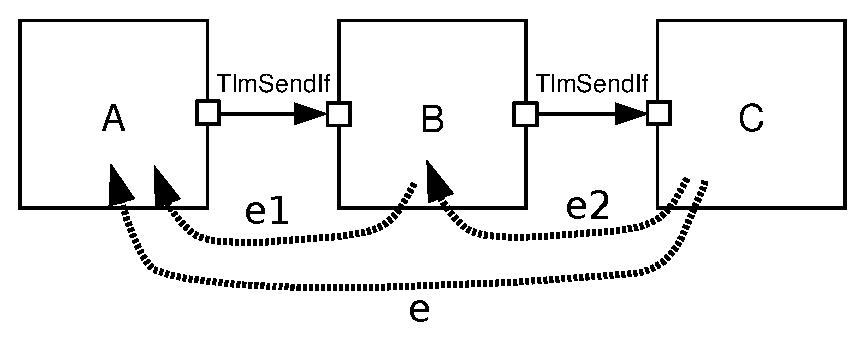
\includegraphics[width=10.0cm]{tlm/chaining_communication_steps.pdf}
    \caption{\label{fig:chaining_communication_steps} Chaining communication steps.}
  \end{center}
\end{figure}

\textbf{Chaining communication steps}. Most of the time a single event
is sufficient for a simple communication scheme. Sometimes several
communication steps are needed before the message actually reachs the
target. For instance, consider an intermediate module is placed
between the initiator and the target,
see~Figure~\ref{fig:chaining_communication_steps}.  Module~A is an
initiator. Module~B is both a target and an initiator. Module~C is a
target. The time spent in module~B affects the total transaction time
between initiator module~A and final target module~C. While the time
spent when processing the transition of the message from A-B to B-C
can be easily computed in module~B \texttt{Send} method, if a single
event is used, the computation of the time spent when the response
goes through B can not be computed, because the response will be
directly notified from module~C to module~A. To account for this
additional delay, only one event is not sufficient. Actually, an
additional event is needed to make module~B wait module~C, while
module~A still waits the target module, which is module~B not
module~C. A stack of events has been introduced to simplify the
programming of chained communication steps. Such communication schemes
are quite common in networks, where intermediate modules would be
switches. Before sending a message, an initiator puts both the request
and the event into the message. Actually, the event is pushed on a
stack. After the \texttt{Send}, the initiator still waits for the
event it has pushed on the stack. Once the event is notified, the
initiator is unblocked and can do a pop on the stack to remove its
event. The TLM interface has been updated to add support for an event
stack, see~Figure~\ref{fig:interface3} (note that access methods to
the stack of events have been omitted from the Figure).

\begin{figure}[h]
  \begin{center}
    \input{tlm/interface3}
    \caption{\label{fig:interface3} TLM interface (with an event stack).}
  \end{center}
\end{figure}

\section{Untimed TLM}
\label{sec:untimed_tlm}

\begin{figure}[h]
  \begin{center}
    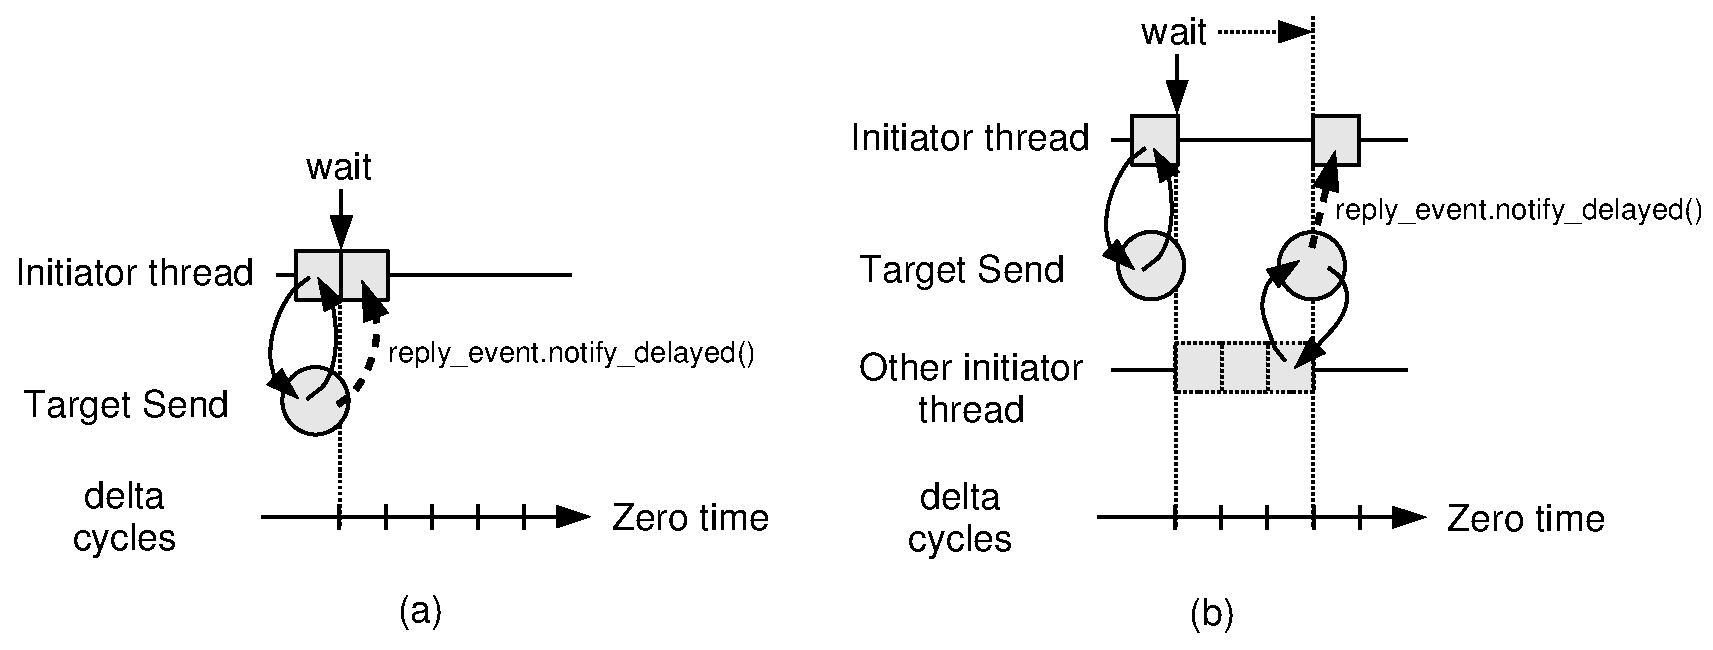
\includegraphics[width=\textwidth]{tlm/utlm_principle.pdf}
    \caption{\label{fig:utlm_principle} Untimed TLM: principle.}
  \end{center}
\end{figure}

This section will demonstrate the use of the TLM interface and message
to design untimed TLM models. In an Untimed TLM (UTLM) model, the
delays for serving requests is not considered,
see~Figure~\ref{fig:utlm_principle}. The simulated time is stuck to
zero and only delta cycles occur during simulation. The initiator
calls target method \texttt{Send} to make the target serve the
request. If the initiator waits for a response, i.e. waits for the
response event, the target triggers the response event for the next
delta cycle, see Figure~\ref{fig:utlm_principle}~(a). While making the initiator wait the response
  event may seem not necessary for untimed models, actually it is necessary
  because the target method \texttt{Send} may not trigger the response
  event before leaving control to the caller initiator thread
  but in another delta cycle. For example, the target may need to receive a
  message from another module to set the response and trigger the
  response event, see Figure~\ref{fig:utlm_principle}~(b).
  As a side effect, forcing this design methodology facilitates the untimed
  and timed models cosimulation, and enables a smooth transition from untimed models to
  timed models.

Consider the example of a system
with one processor and one memory: the processor is an initiator
whereas the memory is a target. Examples of request and response are
provided on Figure~\ref{fig:memory_req_rsp}. The processor can send
\texttt{READ} or \texttt{WRITE} requests to the memory. When the
request is a write, \texttt{MemoryRequest} member \texttt{write\_data}
helds the data to write.

\begin{figure}[p]
\begin{minipage}{\textwidth}
  \begin{center}
    \input{tlm/memory_req_rsp}
    \caption{\label{fig:memory_req_rsp} Example of memory request \& response.}
  \end{center}
\end{minipage}
\begin{minipage}{\textwidth}
~\vspace{3.0cm}
\end{minipage}
\begin{minipage}{\textwidth}
  \begin{center}
    \input{tlm/utlm_memory}
    \caption{\label{fig:utlm_memory} Example of UTLM memory module.}
  \end{center}
\end{minipage}
\end{figure}

A source code example for the processor is provided on
Figure~\ref{fig:utlm_processor}. The processor module has only one
SystemC thread: \texttt{Run}. Thread \texttt{Run} calls
\texttt{PerformRead} and \texttt{PerformWrite} member methods. These
two methods do memory requests using SystemC port \texttt{port}. The
\texttt{PerformRead} operation is the following:

\begin{enumerate}
\item[{\large \ding{202}}] a memory request is allocated;
\item[{\large \ding{203}}] a message is allocated, and initialized
  with the request and the response event;
\item[{\large \ding{204}}] the request is filled;
\item[{\large \ding{205}}] the message is sent using port method
  \texttt{Send}; \texttt{Send} is retried until it has
  succeeded;
\item[{\large \ding{206}}] if \texttt{Send} has failed, the processor
  waits for one delta cycle before actually retrying \texttt{Send};
\item[{\large \ding{207}}] once \texttt{Send} has succeeded, the
  processor waits for the response event;
\item[{\large \ding{208}}] once \texttt{wait} is finished, the
  processor can use the response.
\end{enumerate}

The \texttt{PerformWrite} operation is the following:
\begin{enumerate}
\item[{\large \ding{202}}] a memory request is allocated;
\item[{\large \ding{203}}] a message is allocated, and initialized
  with the request and the response event;
\item[{\large \ding{204}}] the request is filled;
\item[{\large \ding{205}}] the message is sent using port
  \texttt{Send} methods; \texttt{Send} is retried until it has
  succeeded;
\item[{\large \ding{206}}] if \texttt{Send} has failed, the processor
  waits for one delta cycle before actually retrying \texttt{Send};
\end{enumerate}

When \texttt{Send} fails and the processor has to wait for a delta
cycle before retrying (see item {\large \ding{206}} from the previous
operations), the programmer should use a private event to first notify
using \texttt{notify\_delayed} SystemC method and after that, perform
the \texttt{wait}, which effectively provoques a one delta cycle wait.
% We will see later, that \texttt{notify\_delayed} is only necessary
% when writing UTLM models, but not necessary for TTLM models.

\begin{figure}[p]
  \begin{center}
    \input{tlm/utlm_processor}
    \caption{\label{fig:utlm_processor} Example of UTLM processor
      module.}
  \end{center}
\end{figure}

A source code example for the memory is provided on
Figure~\ref{fig:utlm_memory}. The memory module has no thread. The
memory requests are directly served by memory method \texttt{Send}
within the processor module thread. Member method \texttt{Send}
operation is the following:

\begin{enumerate}
\item[{\large \ding{202}}] the request is taken from the message;
\item[{\large \ding{203}}] the response is allocated;
\item[{\large \ding{204}}] if the request is a \texttt{READ}, the
  reponse is filled with the read data; the response is put in the
  message and the response event is notified for the next delta cycle;
\item[{\large \ding{205}}] if the request is a \texttt{WRITE}, the
  data to write is written back in the memory.
\end{enumerate}


\section{Timed TLM}
\label{sec:timed_tlm}

\begin{figure}[h]
  \begin{center}
    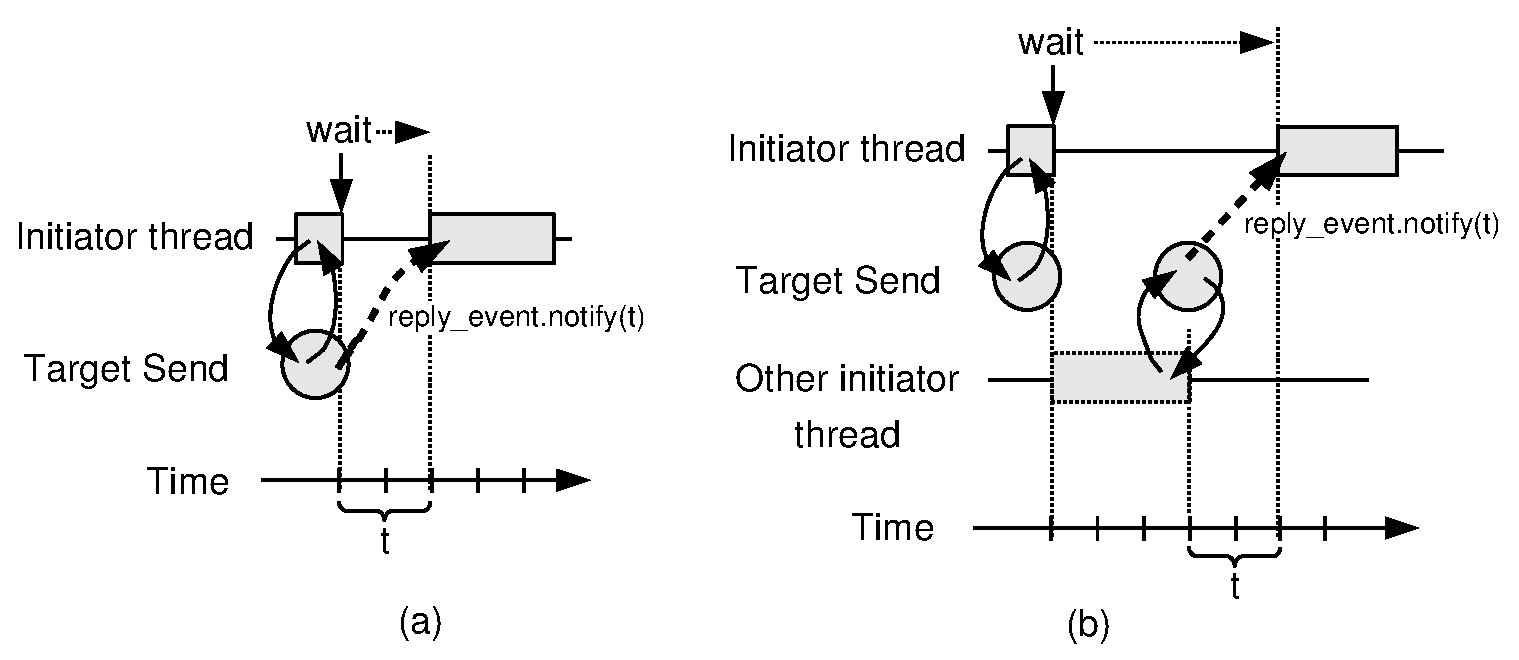
\includegraphics[width=\textwidth]{tlm/ttlm_principle.pdf}
    \caption{\label{fig:ttlm_principle} Timed TLM: principle.}
  \end{center}
\end{figure}

In this section, the use of the TLM interface and message with time
(TTLM) will be demonstrated on several examples with an increasing
complexity. The first example presents how to add time to the untimed
model using one-to-one communication scheme, see
section~\ref{sec:untimed_tlm}. The next example presents a N-to-M
communication scheme using a router between the processors and the
memory, and applying contention over the processors requests. The last
example presents an N-to-M communication scheme using a router between
the processors and the memories, and applying contention over
processors requests and memories responses. As several
processors/memories compete for accessing to the router, the router is
using an arbitration algorithm.  The arbitration algorithm assigns a
fixed time slot to each processor/memory.

In the proposed model the initiator must place itself in the right
time when sending a request, i.e., calling the \texttt{Send} method.
For that purpose, the initiator must use the \texttt{wait} method.
When the target needs to reply to a request the \texttt{notify} method
is used over the response event with the estimated time taken by the
target, see Figure~\ref{fig:ttlm_principle}. The target module
  can trigger the response event when executing the \texttt{Send}
  method, i.e., in the initiator thread, see
  Figure~\ref{fig:ttlm_principle}~(a); or during another cycle (or
  delta cycle), for example, the target module may need that another
  initiator module sends a message to it before triggering the first
  initiator response event, see Figure~\ref{fig:ttlm_principle}~(b).
Note that unlike in the UTLM model \texttt{notify\_delayed} is no
longer needed, unless the notification takes zero time.

\subsection{Example: Simple Model}
The modifications to the UTLM example to make it TTLM are minimal.
Processor and memory now have time parameters among their template
parameters (i.e., \texttt{FREQUENCY} and \texttt{READ\_CYCLES}), which
are used to compute the processor and memory processing times.

The main modification in the processor module is the substitution and
addition of calls to the SystemC primitive \texttt{wait} with time,
see {\large \ding{202}} and {\large \ding{203}} on
Figure~\ref{fig:ttlm_processor}\footnote{This implementation is
  innefficient, because a call to the \texttt{wait} method is done
  (that is, a SystemC synchronization) for each executed instruction.
  Better implementations can be done, but this is not the objective of
  this example.}. For example, it is used when trying to send a
read/write request, and the request fails, see {\large \ding{202}} on
Figure~\ref{fig:ttlm_processor}.  Another use is to advance the
internal clock of the module after an instruction execution, see
{\large \ding{203}} on Figure~\ref{fig:ttlm_processor}.

To convert the memory module to a TTLM module, we have only modified
the call to the \texttt{notify} method, see {\large \ding{202}} on
Figure~\ref{fig:ttlm_memory}, to indicate the time the memory needs to
set the response, the response delay time. Note that the memory sets
the response before notifying it, and that the response could be used
before the delay time, however the module that receives the response
should never suppose so, i.e., another implementation of the memory
could have wait the delay time before setting the response and simply
make a \texttt{notify\_delayed} to make it available.

\begin{figure}[p]
  \begin{center}
    \input{tlm/ttlm_processor}
    \caption{\label{fig:ttlm_processor} Example of TTLM processor.}
  \end{center}
\end{figure}

\begin{figure}[p]
\begin{minipage}{\textwidth}
  \begin{center}
    \input{tlm/ttlm_memory}
    \caption{\label{fig:ttlm_memory} Example of TTLM memory.}
  \end{center}
\end{minipage}
\begin{minipage}{\textwidth}
~\vspace{2.5cm}
\end{minipage}
\begin{minipage}{\textwidth}
  \begin{center}
    \input{tlm/ttlm_router}
    \caption{\label{fig:ttlm_router} Untimed implementation of the
      \texttt{router} module.}
  \end{center}
\end{minipage}
\end{figure}


\subsection{Example: Request contention}
\label{subsec:example_request_contention}

\begin{figure}[h]
  \begin{center}
    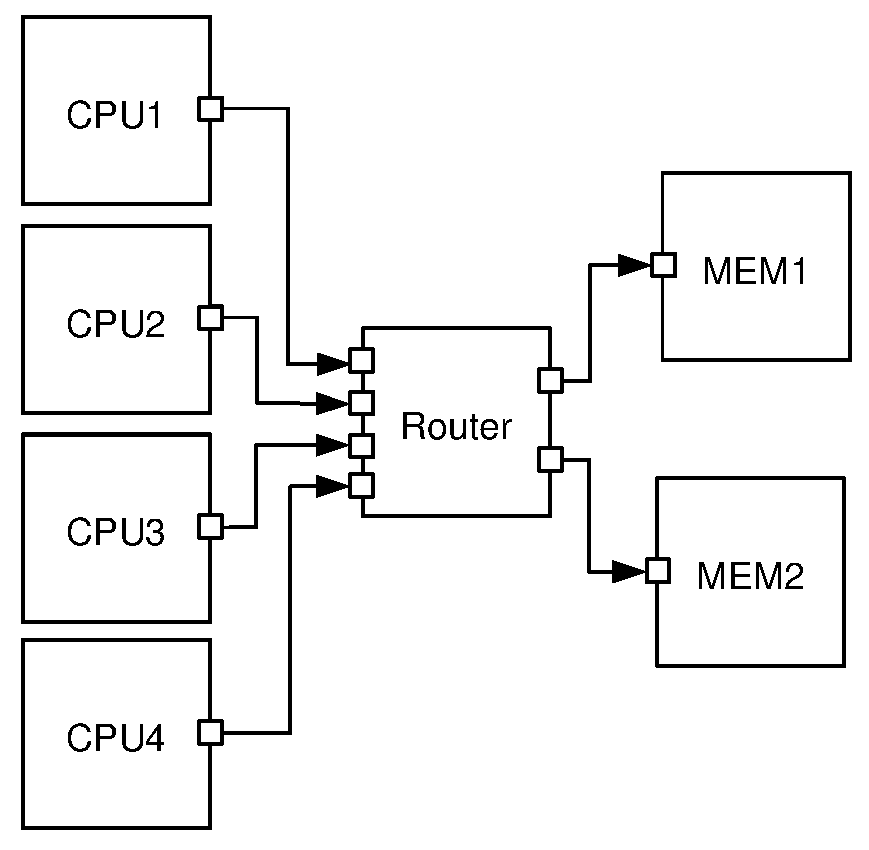
\includegraphics[width=7.0cm]{tlm/n_to_m.pdf}
    \caption{\label{fig:n_to_n} M-initiators~x~N-targets.}
  \end{center}
\end{figure}

This example shows how a module can perform contention over the
request. For that purpose a new module is added: the \texttt{router}
module which connects the processors to multiple memories, see
Figure~\ref{fig:n_to_n}. For a simple untimed implementation of the
\texttt{router} module see Figure~\ref{fig:ttlm_router}. This
implementation does not make any contention over the incomming
requests, neither over responses. This example is going to show how to
implement contention over the incomming requests, later
Section~\ref{subsec:example_response_contention} will show how to
implement contention over the responses.

The \texttt{router} module implements a round robin scheduling
algorithm to give access to the memories, i.e., if two processors are
simulated processor 0 has access to the memories during cycles 0, 2,
4,\ldots , and processor 1 at cycles 1, 3, 5,\ldots.
Figure~\ref{fig:ttlm_router_adv} shows a possible implementation. In
this implementation, the \texttt{router} module is a hierarchical
module that associates to each input port a \texttt{MasterPortModule}
module which actually implements the contention, see {\large
  \ding{202}} on Figure~\ref{fig:ttlm_router_adv}.

\texttt{MasterPortModule} bufferizes all the incomming requests and
dispatches them in the incomming order during the time windows
associated to the port using a thread. This module implements the
\texttt{Send} method from the \texttt{TlmSendIf} interface to handle
incomming requests, see {\large \ding{202}} and {\large \ding{203}} on
Figure~\ref{fig:ttlm_router_adv}. A buffer holds incomming requests
and the \texttt{Dispatch} thread of the module dispatches them to the
right output port during the time windows of the incomming port, see
{\large \ding{204}} on Figure~\ref{fig:ttlm_router_adv}.  To execute
the \texttt{Dispatch} process at the right time windows the
\texttt{dispatch\_event} (from which the \texttt{Dispatch} process
depends) has to be carefully triggered. In this example, the
\texttt{dispatch\_event} is triggered with the right delay when a new
request is queued (note that time can be equal to zero, which means
that the event will be notified during the next delta cycle, but the
SystemC clock will not be modified), see {\large \ding{205}} on
Figure~\ref{fig:ttlm_router_adv}. In case the buffer is not empty
after dispatching the oldest request (or if the oldest request has not
been accepted) another \texttt{dispatch\_event} is triggered, to
execute the \texttt{Dispatch} thread during the next time window and
send pending requests, see {\large \ding{206}} on
Figure~\ref{fig:ttlm_router_adv}.


\subsection{Example: Response contention}
\label{subsec:example_response_contention}
Section~\ref{subsec:example_request_contention} showed how contention
can be done over incomming requests. However, in many situations
contention over the responses is also desired. This example, modifies
the previously shown \texttt{router} with requests contention to
support contention over responses. For the new implementation of the
\texttt{router} see Figure~\ref{fig:ttlm_router_adv2}.

The \hfill hierarchical \hfill \texttt{router} \hfill module \hfill contains \hfill the \hfill definition \hfill of \hfill an \hfill additional \hfill module: the \texttt{SlavePortController} module, see
{\large \ding{202}} on Figure~\ref{fig:ttlm_router_adv2}. An instance
of this module is associated to each output port, and connected to
each of the instances of \texttt{MasterPortController}.

To easily handle multiple responses it implements the
\texttt{ResponseReceived} method from the \texttt{ResponseListener}
utility class (included in the source distribution of the TLM model
presented in this document), see {\large \ding{203}} and {\large
  \ding{204}} on Figure~\ref{fig:ttlm_router_adv2}.  Conceptually, the
\texttt{ResponseListener} utility class allows to send a message
through a port with the \texttt{Send} method provided by this class,
and be notified when the response is received thanks to the
\texttt{ResponseReceived} method.

The \texttt{SlavePortController} also implements the \texttt{Send}
method from the \texttt{TlmSendIf} interface to handle requests
comming from the \texttt{MasterPortController} modules, see {\large
  \ding{203}} and {\large \ding{205}} on
Figure~\ref{fig:ttlm_router_adv2}. The \texttt{Send} method checks if
the request requires a response:
\begin{itemize}
\item if not it just forwards the request to the output port, see
  {\large \ding{206}} on Figure~\ref{fig:ttlm_router_adv2};
\item if a response is required then it uses the \texttt{Send} method
  provided by the \texttt{ResponseListener} class to forward send the
  request through the output port, and be notified (through the
  \texttt{ResponseReceived} method when the response is available, see
  {\large \ding{207}} on Figure~\ref{fig:ttlm_router_adv2}.
\end{itemize}

When a response to a message is received the
\texttt{SlavePortController} handles it as the
\texttt{MasterPortController}, that is, it puts the message in a
buffer and dispatches it with the \texttt{Dispatch} thread during the
time windows given to the port, see {\large \ding{208}} on
Figure~\ref{fig:ttlm_router_adv2}.

\begin{figure}[p]
  \begin{center}
    \input{tlm/ttlm_router_adv}
    \caption{\label{fig:ttlm_router_adv} Example of TTLM router module
      with requests contention.}
  \end{center}
\end{figure}

\begin{figure}[p]
  \begin{center}
    \input{tlm/ttlm_router_adv2}
    \caption{\label{fig:ttlm_router_adv2} Example of TTLM router
      module with requests and responses contention.}
  \end{center}
\end{figure}


\begin{appendix}
\chapter{TLM library}
\label{tlm_appendix}
\section{The message}
\section{The \texttt{ResponseListener} class}


\end{appendix}

% \input{filename}
% \begin{appendix}
% \input{filename} 
% \end{appendix}
\bibliographystyle{plain}
\bibliography{biblio}


\end{document}
